\chapter{Algorithm and Implementation}
In this chapter, we'll look into the algorithm overview and the corresponding implementation details.

\section{Generating Particles}
\begin{figure}[htp]
\begin{center}
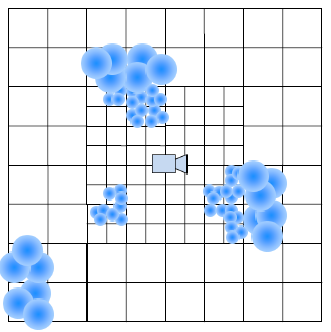
\includegraphics[scale=0.5]{images/particlegrid.png}
\caption{Camera-centered particle grid}
\label{f13}
\end{center}
\end{figure}

The author proposed with an interesting fully procedural method to generate the particles using a camera-centered particle grid shown above. 
\subsection{The Design}
This grid has several cells, each one containing several particle layers. The number of the layers, the particle size and the density are determined by 2D noise texture. Usually, the particles in each next ring have twice the size of the inner ring.\\\\\\\\

\begin{figure}[htp]
\begin{center}
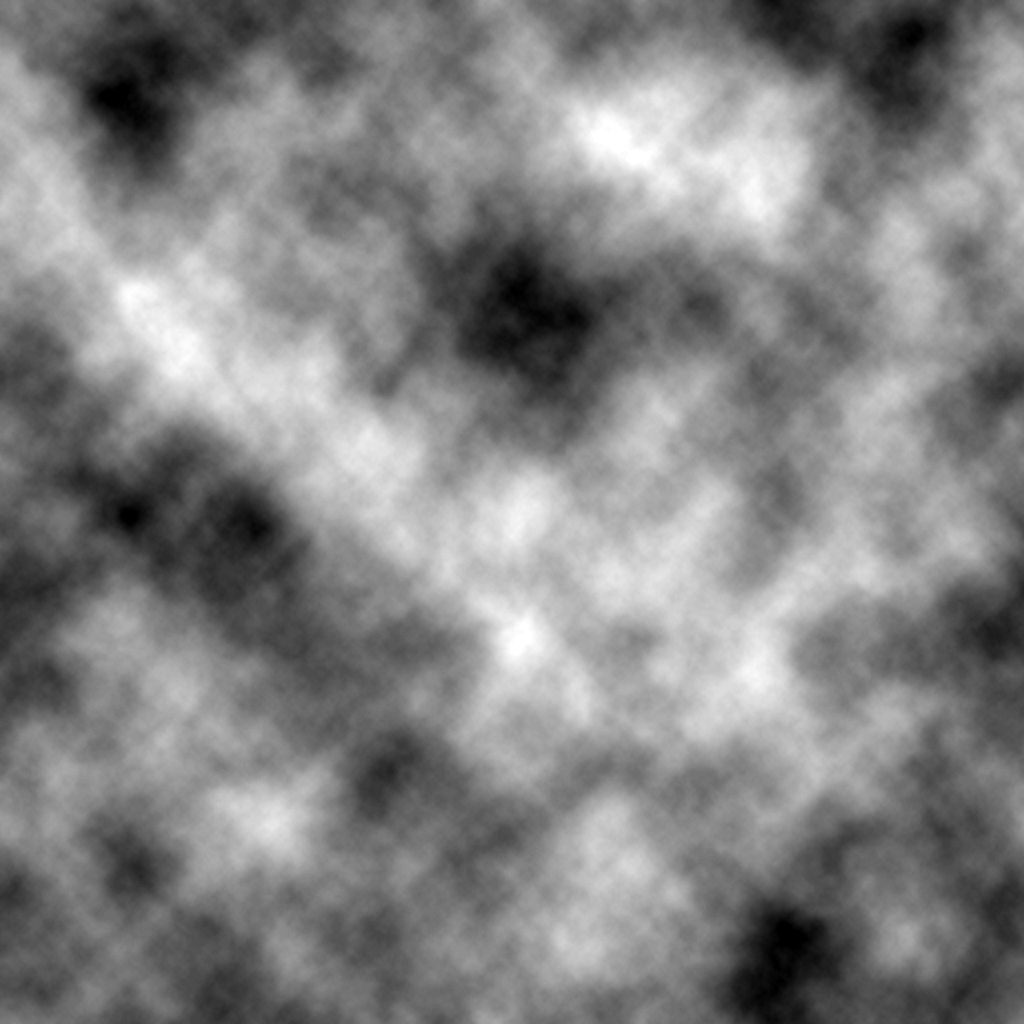
\includegraphics[scale=0.1]{images/Noise.png}
\caption{A typical noise texture}
\label{f10}
\end{center}
\end{figure}

\subsection{The Implementation}
The generation process is performed on GPU by the following steps:
\begin{enumerate}
\item Process each cell, compute the cloud density of this cell, and create a list of valid non-empty cells according to the 2D noise texture. In this step, one shader thread process one cell, and a buffer is used to store the indices of valid cells.
\item Process the list of valid cells from the previous step. Generate one or more particles for each cell depending on the number of the layers and cloud density in the cell. In this step, one shader thread process one valid cell and generates particles.
\item Generate an ordered list of particles because they must be rendered in back to front order for the blending purpose. However, sorting on GPU is quite expensive, so the author provided a solution that using streaming output the particles only for valid cells to preserve the order, and then process 32 particles by one GS thread.
\end{enumerate}
\section{Pre-Computing 4D Look-up Tables}
The current graphics hardware does not support 4D textures, so the author used 3D textures with manual interpolation for the forth coordinate to emulate the 4D texture. 

\subsection{The Design}
The optical depth integral is stored in a $64\times 32\times 64\times 32$ 8-bit look-up table which occupies 4 MB storage space. Single and multiple scattering are stored in two $32\times 64\times 16\times 8$ 16-bit float look-up tables. Each table occupies 0.5 MB storage space.
\subsection{The Implementation}
\begin{lstlisting}
#define SAMPLE_4D_LUT(tex3DLUT, LUT_DIM, f4LUTCoords, fLOD, Result) 
{                                                              
    float3 f3UVW;                                              
    f3UVW.xy = f4LUTCoords.xy;                                 
    float fQSlice = f4LUTCoords.w * LUT_DIM.w - 0.5;           
    float fQ0Slice = floor(fQSlice);                           
    float fQWeight = fQSlice - fQ0Slice;                       
                                                               
    f3UVW.z = (fQ0Slice + f4LUTCoords.z) / LUT_DIM.w;          
    /* frac() assures wraparound filtering of w coordinate*/ 
    Result = lerp(tex3DLUT.SampleLevel(samLinearWrap, f3UVW, fLOD), 									 tex3DLUT.SampleLevel(samLinearWrap, frac(f3UVW + float3(0,0,1LUT_DIM.w)), 					 fLOD), fQWeight);                                                                          
}
\end{lstlisting}
As we can see in the code snippet above, \textbf{SAMPLE\_4D\_LUT} is a utility function which returns an interpolated result into the 5th parameter from the first 4 parameters, which are 3D texture, dimension, coordinates and LOD index.
\section{Pre-Computing Optical Depth}
The first step is to pre-compute the optical depth using Equation 2.2: $\tau(A, B) = \int_{A}^{B}\beta(P)\cdot ds$ for each ray to the boundary of a certain particle. The author assumed that the camera will always stay outside the volume. Then, the goal of this step is to calculate the optical depth integral for all possible camera positions and orientations.

\begin{figure}[htp]
\begin{center}
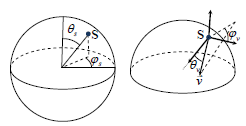
\includegraphics[scale=1.0]{images/startandview.png}
\caption{Four angels to describe a ray}
\label{f8}
\end{center}
\end{figure}

\subsection{The Design}
To describe a ray, we need 4 angles, 2 angles describing the start point on the particle sphere, and 2 angles describing the view direction. Because of the 4 parameters, a 4D look-up table is necessary. As shown in the figure above, $\varphi_S\in[0, 2\pi]$ and $\theta_S\in[0, \pi]$ are used to specify the start point of the ray. While $\varphi_v\in[0, 2\pi]$ and $\theta_v\in[0, \frac{\pi}{2}]$ are used to specify the direction of the ray.

\begin{figure}[htp]
\begin{center}
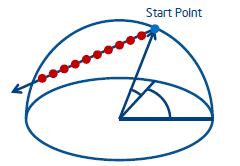
\includegraphics[scale=0.8]{images/opticaldepthintegration.png}
\caption{Numerically integrate the optical depth of a ray}
\label{f9}
\end{center}
\end{figure}

Then we use Equation 2.2: $\tau(A, B) = \int_{A}^{B}\beta(P)\cdot ds$ to accumulate the optical depth of a ray. Now, here is the interesting part of how to retrieve the extinction coefficient $\beta(P)$. The author used 4D look-tables which contains several 3D noises to get the extinction coefficient. The figure below shows one typical noise texture.

\subsection{The Implementation}
After carefully explaining the design of the first step, let's have a look at how the actual related function in the shader looks like. Please note that the rendering API is \textbf{DirectX}, hence the shader is written in \textbf{HLSL}.
\begin{lstlisting}
// This shader computes level 0 of the maximum density mip map
float2 PrecomputeOpticalDepthPS(SScreenSizeQuadVSOutput In) : SV_Target
{
    float3 f3NormalizedStartPos, f3RayDir;
    OpticalDepthLUTCoordsToWorldParams( float4(ProjToUV(In.m_f2PosPS), g_GlobalCloudAttribs.f4Parameter.xy), f3NormalizedStartPos, f3RayDir );
    
    // Intersect view ray with the unit sphere:
    float2 f2RayIsecs;
    // f3NormalizedStartPos  is located exactly on the surface; slightly move start pos inside the sphere
    // to avoid precision issues
    GetRaySphereIntersection(f3NormalizedStartPos + f3RayDir*1e-4, f3RayDir, 0, 1.f, f2RayIsecs);
    
    if( f2RayIsecs.x > f2RayIsecs.y )
        return 0;

    float3 f3EndPos = f3NormalizedStartPos + f3RayDir * f2RayIsecs.y;
    float fNumSteps = NUM_INTEGRATION_STEPS;
    float3 f3Step = (f3EndPos - f3NormalizedStartPos) / fNumSteps;
    float fTotalDensity = 0;
    float fDistToFirstMatter = -1;
    for(float fStepNum=0.5; fStepNum < fNumSteps; ++fStepNum)
    {
        float3 f3CurrPos = f3NormalizedStartPos + f3Step * fStepNum;
        
        float fDistToCenter = length(f3CurrPos);
        float fMetabolDensity = GetMetabolDensity(fDistToCenter);
        float fDensity = 1;
#if DENSITY_GENERATION_METHOD == 0
        fDensity = saturate( 1.0*saturate(fMetabolDensity) + 1*pow(fMetabolDensity,0.5)*(GetRandomDensity(f3CurrPos, 0.15, 4, 0.7 )) );
#elif DENSITY_GENERATION_METHOD == 1
        fDensity = 1.0*saturate(fMetabolDensity) + 1.0*pow(fMetabolDensity,0.5)*(GetRandomDensity(f3CurrPos, 0.1,4,0.8)) > 0.1 ? 1 : 0;
#elif DENSITY_GENERATION_METHOD == 2
        fDensity = GetPyroSphereDensity(f3CurrPos);
#endif

        if( fDensity > 0.05 && fDistToFirstMatter < 0 )
            fDistToFirstMatter = fStepNum / fNumSteps;
       
        fTotalDensity += fDensity;
    }
    if( fDistToFirstMatter < 0 ) fDistToFirstMatter = 1;
    return float2(fTotalDensity / fNumSteps, fDistToFirstMatter);
}
\end{lstlisting}


The integration function is \textbf{PrecomputeOpticalDepthPS}. Firstly, it decomposes the given projection position and the 4 angle parameters from inhomogeneous coordinates into 2 vec3 positions, the first one \textbf{f3NormalizedStartPos} describes the start position of the ray, the second one \textbf{f3RayDir} describes the ray direction. Then the intersecting view ray inside the unit sphere is calculated. Since the start position is just on the surface of the sphere, in order to avoid precision issues, the author moved the start position slightly into the sphere by the amount of \textbf{f3RayDir*1e-4}. Then the integration is done inside the \textbf{for loop}. \textbf{DENSITY\_GENERATION\_METHOD} is defined as: 0 represents radial fall-off + 3D noise, 1 represents 3D noise + thresholding, 2 represents pyroclastic style.
\textbf{fDensity} is the current density of this step. Finally, the total density \textbf{fTotalDensity} for a ray is accumulated.


\section{Pre-Computing Scattering}
In this step, the author proposed with two types of scattering: single scattering and multiple scattering. In nature, a photon inside a cloud is scattered multiple times before it leaves the cloud. Hence the author concentrated on the multiple scattering in order to render a realistic cloud appearance. The goal is to calculate multiple scattering for every possible light position, camera position and orientation.

\subsection{Single Scattering}
\subsubsection{The Design}
\begin{figure}[htp]
\begin{center}
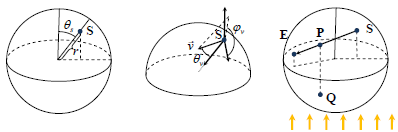
\includegraphics[scale=1.0]{images/singlescattering.png}
\caption{Pre-computing single scattering inside the spherical
particle}
\label{f11}
\end{center}
\end{figure}
First of all, the author assumed that the particle density only depends on the distance to the center. As the particle is a perfect sphere, which has the nature of symmetry, the author indicated that an arbitrary light direction coinciding with positive $z$ axis can be chosen to examine one of the rays that intersect the sphere. Since the light field is also symmetrical, only one angle $\theta_S$ is needed to describe the start point of a ray. As discussed in the previous section, another 2 angles $\phi_v$ and $\theta_v$ will still be needed to describe the ray direction. As the light field inside the volumes is important to solve the scattering equation, the author introduced a 4D look-up table with 3 angles($\theta_S$, $\phi_v$ and $\theta_v$) and the fraction of distance $r$ from the center of the sphere. We denote the table by 
\begin{equation}
\overline{L}^{(1)}_{In}(\theta_S, \phi_v, \theta_v, r), \theta_S\in[0, \pi], \phi_v\in[0, \pi], \theta_v\in[0, \pi], r\in[0, 1].
\end{equation}
The author then proposed with a solution to single scattering inside the spherical particle:
\begin{equation}
\overline{L}^{(1)}_{In} = \int_{S}^{E}e^{-\tau(P,S)}e^{-\tau(P,Q)} \cdot \beta(P) \cdot ds,
\end{equation}
where \textbf{S} is the start point of the ray and \textbf{E} is the exit point of the ray. \textbf{Q} is the point on the surface of the sphere through which the light reaches the current integration point \textbf{P}. The author finally implied that the phase function $P(\theta)$ is only used at run time to avoid precision issues. Just like the optical depth calculation, the extinction coefficient $\beta(P)$ can be evaluated in different methods as long as the distance to the center is the only influencing factor. The author tried different methods and finally decided to make the density constant.

\subsubsection{The Implementation}
Let's have a look at the implementation detail in code.
\begin{lstlisting}
float PrecomputeSingleSctrPS(SScreenSizeQuadVSOutput In) : SV_Target
{
    float4 f4LUTCoords = float4(ProjToUV(In.m_f2PosPS), g_GlobalCloudAttribs.f4Parameter.xy);
    float3 f3EntryPointUSSpace, f3ViewRayUSSpace, f3LightDirUSSpace;
    float fDensityScale;
    ParticleScatteringLUTToWorldParams(f4LUTCoords, g_GlobalCloudAttribs.f4Parameter.z, f3EntryPointUSSpace, f3ViewRayUSSpace, f3LightDirUSSpace, false, fDensityScale);
    // Intersect view ray with the unit sphere:
    float2 f2RayIsecs;
    // f3NormalizedStartPos  is located exactly on the surface; slightly move the start pos inside the sphere
    // to avoid precision issues
    float3 f3BiasedEntryPoint = f3EntryPointUSSpace + f3ViewRayUSSpace*1e-4;
    GetRaySphereIntersection(f3BiasedEntryPoint, f3ViewRayUSSpace, 0, 1.f, f2RayIsecs);
    if( f2RayIsecs.y < f2RayIsecs.x ) return 0;
    float3 f3EndPos = f3BiasedEntryPoint + f3ViewRayUSSpace * f2RayIsecs.y;
    float fNumSteps = NUM_INTEGRATION_STEPS;
    float3 f3Step = (f3EndPos - f3EntryPointUSSpace) / fNumSteps;
    float fStepLen = length(f3Step);
    float fCloudMassToCamera = 0;
    float fParticleRadius = GetParticleSize(GetCloudRingWorldStep(0, g_GlobalCloudAttribs));
    float fInscattering = 0;
    for(float fStepNum=0.5; fStepNum < fNumSteps; ++fStepNum)
    {
        float3 f3CurrPos = f3EntryPointUSSpace + f3Step * fStepNum;
        float fDensity = 1;
        fDensity *= fDensityScale;
        float fCloudMassToLight = 0;
        GetRaySphereIntersection(f3CurrPos, f3LightDirUSSpace, 0, 1.f, f2RayIsecs);
        if( f2RayIsecs.y > f2RayIsecs.x )
        {
            fCloudMassToLight = abs(f2RayIsecs.x) * fParticleRadius;
        }
        float fTotalLightAttenuation = exp( -g_GlobalCloudAttribs.fAttenuationCoeff * (fCloudMassToLight + fCloudMassToCamera) );
        fInscattering += fTotalLightAttenuation * fDensity * g_GlobalCloudAttribs.fScatteringCoeff;
        fCloudMassToCamera += fDensity * fStepLen * fParticleRadius;
    }
    return fInscattering * fStepLen * fParticleRadius;
}
\end{lstlisting}


Similar to the function calculating optical depth, this function \textbf{PrecomputeSingleSctrPS} firstly decomposes the given projection position and the 4 parameters from the 4D look-up table into 3 vec3 positions: the first one \textbf{f3EntryPointUSSpace} describes the start position of the ray, the second one \textbf{f3ViewRayUSSpace} describes the ray direction, the last one \textbf{f3LightDirUSSpace} describes the light direction. Using these 3 components, the density scale is calculated. Similarly, the intersection view ray is evaluated carefully avoiding the precision issues by moving the starting point slightly into the sphere by the amount of \textbf{f3ViewRayUSSpace*1e-4}. Then the integration is performed in the \textbf{for loop}. In each step, we calculate the distance \textbf{fCloudMassToLight} from center of the cloud to the light, and the distance \textbf{fCloudMassToCamera} from the center of the cloud to the camera. Then we can evaluate the total light attenuation \textbf{fTotalLightAttenuation}. Finally, we accumulate the single scattering result \textbf{fInscattering} and \textbf{fCloudMassToCamera} because we are moving forward. Why didn't the author accumulate \textbf{fCloudMassToLight}? That's because the light source is treated as directional light, which means the light source is in an infinite distance.

\subsection{Multiple Scattering}
Multiple scattering is based single scattering using Equation 3.2 $\overline{L}^{(1)}_{In} = \int_{S}^{E}e^{-\tau(P,S)}e^{-\tau(P,Q)} \cdot \beta(P) \cdot ds$. However, this time, we need to calculate $\overline{L}^{(n)}_{In}$.
\subsubsection{The Design}
The author proposed with 3 steps:
\begin{enumerate}
\item Evaluate $\overline{J}^{(n)}(\theta_S, \phi_v, \theta_v, r)$  for every point and direction inside he sphere by solving Equation 2.8: $J^{(n)}(P, \vec{v}) = \int_{\Omega}L_In(P, \vec{\omega}) \cdot P(\theta) \cdot d\omega$.
\item Evaluate $\overline{L}_{In}^{(n)}(\theta_S, \phi_v, \theta_v, r)$ as the current order in scattering by solving Equation 2.7: $L_{In}^{(n)}(C, \vec{v}) = \int_{P_0}^{P_1}e^{-\tau(P, P_0)} \cdot J(P, \vec{v}) \cdot \beta(P) \cdot ds$.
\item Accumulate current scattering order to the total look-up table: $\overline{L}_{In}^M = \overline{L}_{In}^M + \overline{L}_{In}^{(n)}$.
\end{enumerate}
As a result, the figure below shows single, multiple and final lighting for the sphere.
\begin{figure}[htp]
\begin{center}
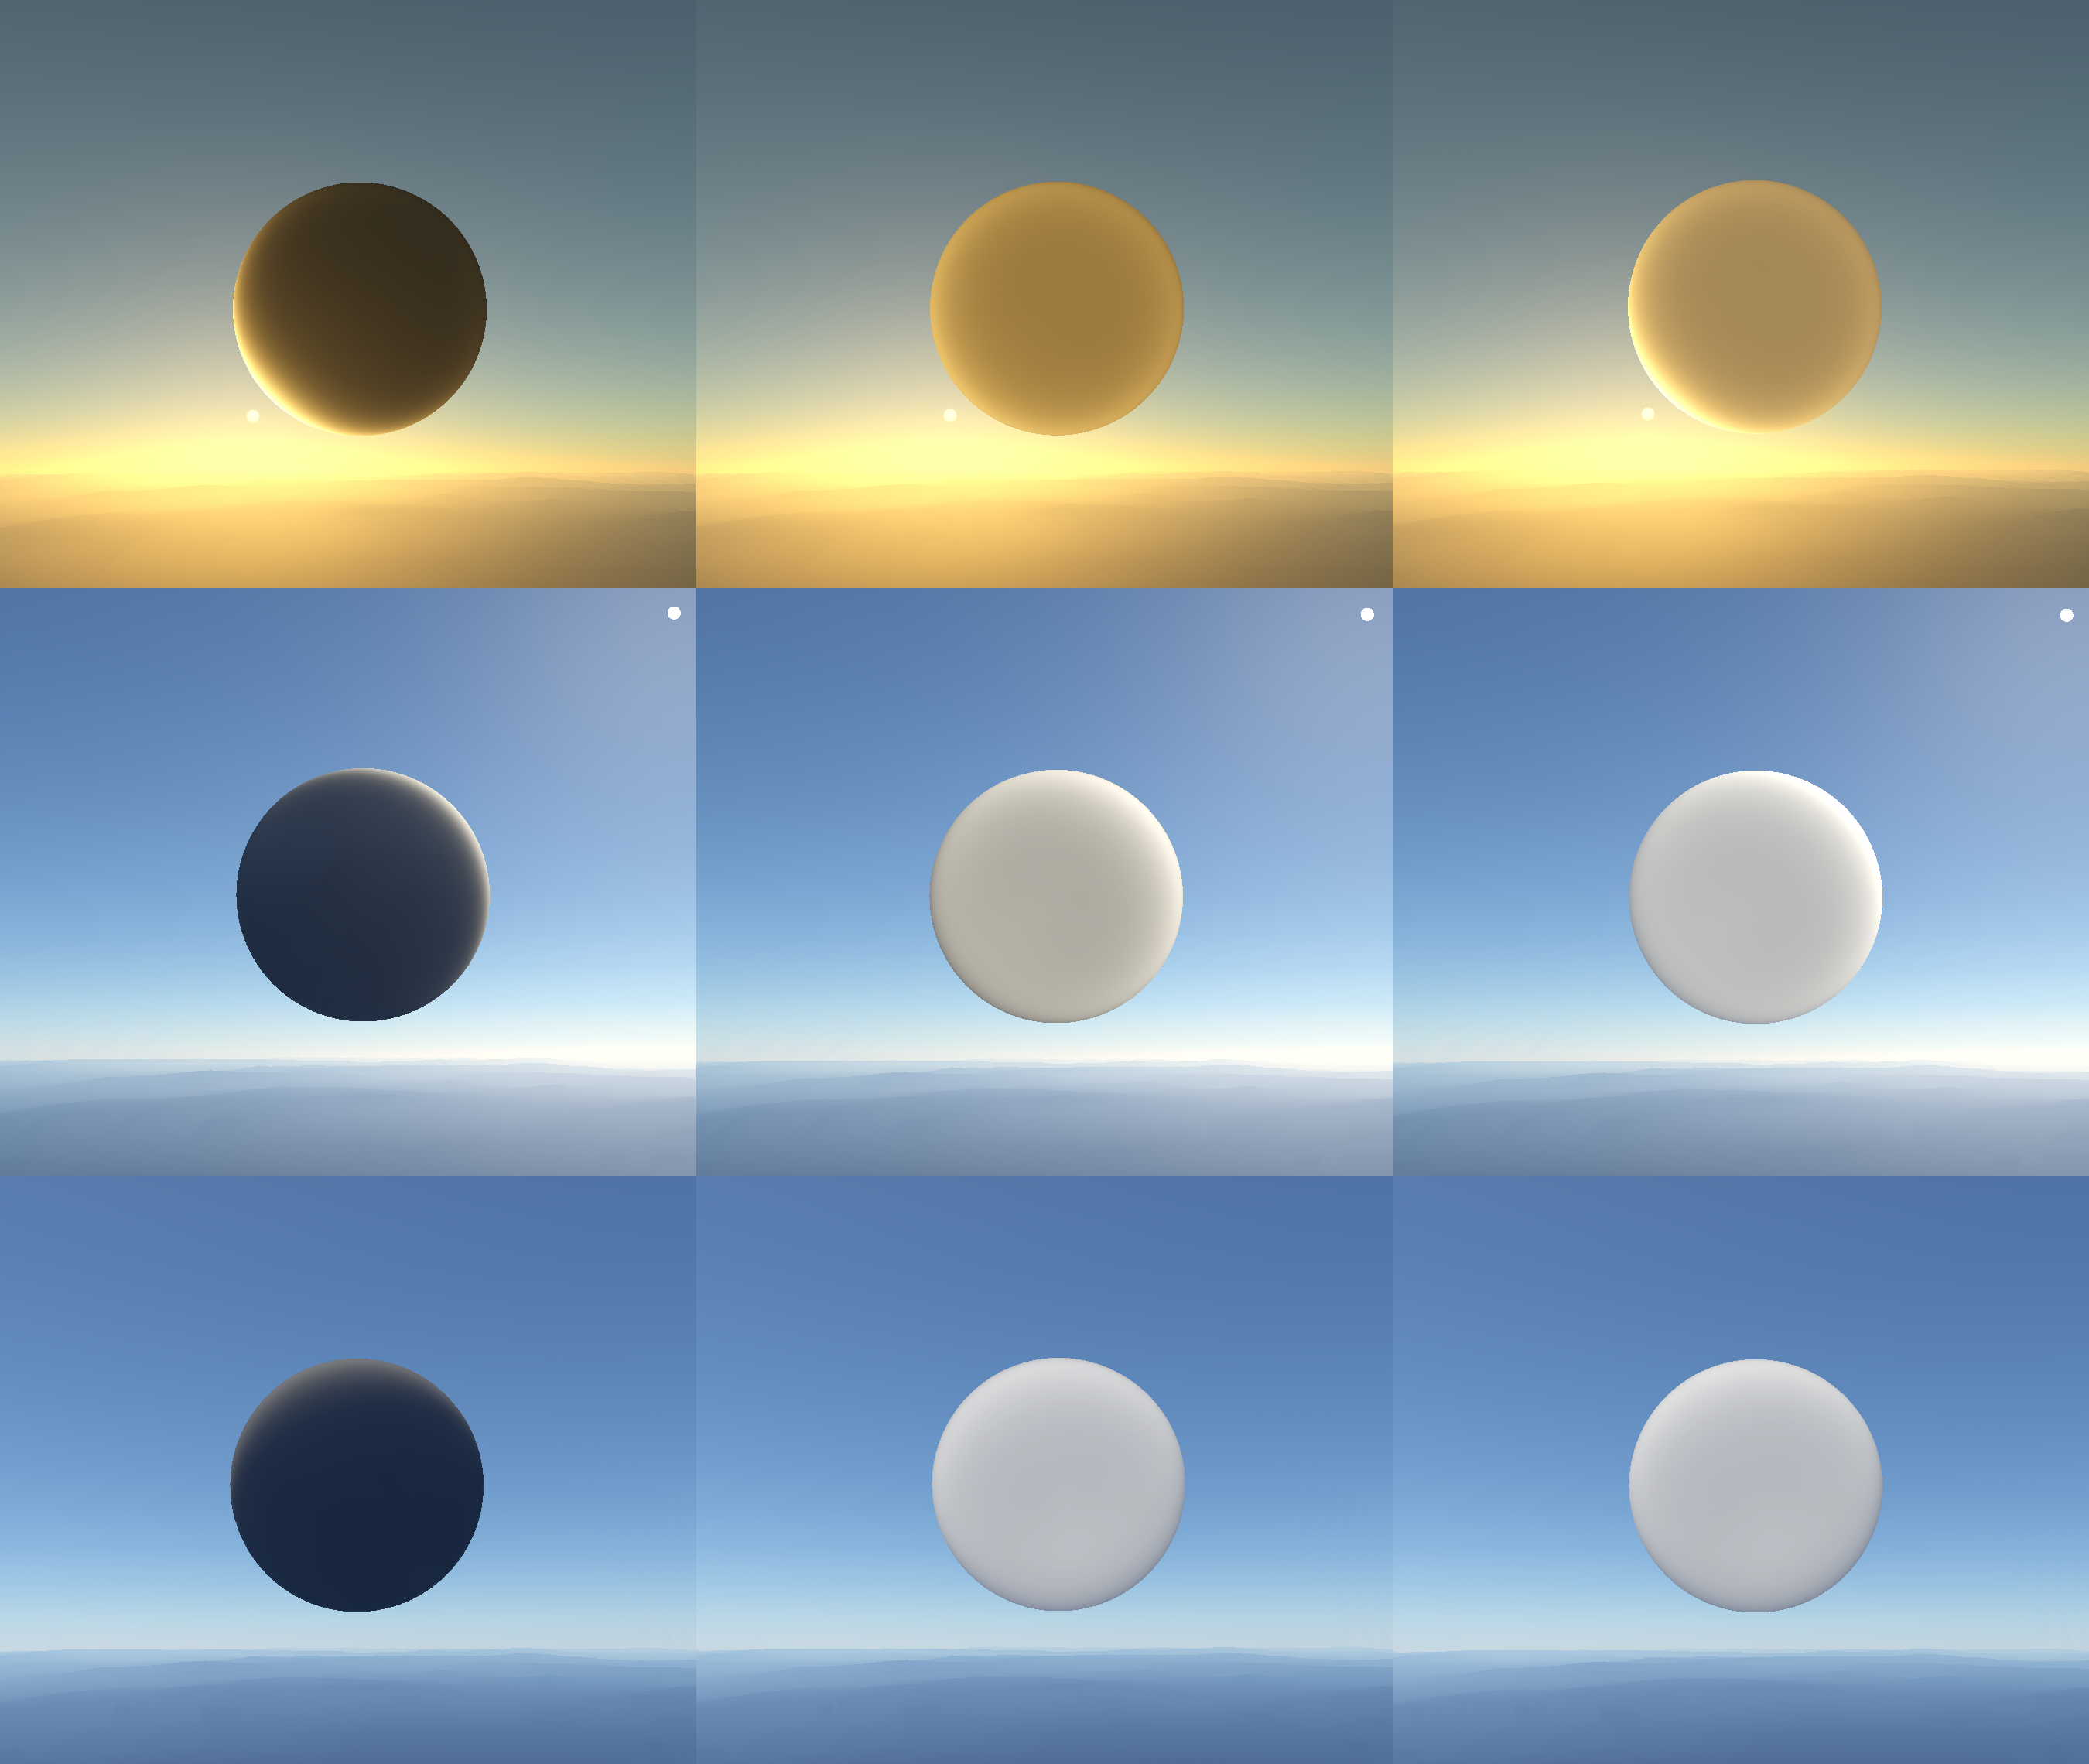
\includegraphics[scale=0.1]{images/scatteringresult.png}
\caption{Pre-computed scattering for different light orientations.
From left to right: single scattering only, 2 + scattering
only, all terms (including ambient). The particle in the bottom
row is illuminated from above}
\label{f12}
\end{center}
\end{figure}
\subsubsection{The Implementation}
We'll look into the implementation details of the 3 steps in this section.
\begin{enumerate}
\item Compute $\overline{J}^{(n)}$ for each point and direction inside the sphere.
\begin{lstlisting}
float GatherScatteringPS(SScreenSizeQuadVSOutput In) : SV_Target
{
    float4 f4LUTCoords = float4(ProjToUV(In.m_f2PosPS), g_GlobalCloudAttribs.f4Parameter.xy);

    float3 f3PosUSSpace, f3ViewRayUSSpace, f3LightDirUSSpace;
    ParticleScatteringLUTToWorldParams(f4LUTCoords, f3PosUSSpace, f3ViewRayUSSpace, f3LightDirUSSpace, false);

    float3 f3LocalX, f3LocalY, f3LocalZ;
    ConstructLocalFrameXYZ(-normalize(f3PosUSSpace), f3LightDirUSSpace, f3LocalX, f3LocalY, f3LocalZ);

    float fGatheredScattering = 0;
    float fTotalSolidAngle = 0;
    const float fNumZenithAngles = VOL_SCATTERING_IN_PARTICLE_LUT_DIM.z;
    const float fNumAzimuthAngles = VOL_SCATTERING_IN_PARTICLE_LUT_DIM.y;
    const float fZenithSpan = PI;
    const float fAzimuthSpan = 2*PI;
    for(float ZenithAngleNum = 0.5; ZenithAngleNum < fNumZenithAngles; ++ZenithAngleNum)
        for(float AzimuthAngleNum = 0.5; AzimuthAngleNum < fNumAzimuthAngles; ++AzimuthAngleNum)
        {
            float ZenithAngle = ZenithAngleNum/fNumZenithAngles * fZenithSpan;
            float AzimuthAngle = (AzimuthAngleNum/fNumAzimuthAngles - 0.5) * fAzimuthSpan;
            float3 f3CurrDir = GetDirectionInLocalFrameXYZ(f3LocalX, f3LocalY, f3LocalZ, ZenithAngle, AzimuthAngle);
            float4 f4CurrDirLUTCoords = WorldParamsToParticleScatteringLUT(f3PosUSSpace, f3CurrDir, f3LightDirUSSpace, false);
            float fCurrDirScattering = 0;
            SAMPLE_4D_LUT(g_tex3DPrevSctrOrder, VOL_SCATTERING_IN_PARTICLE_LUT_DIM, f4CurrDirLUTCoords, 0, fCurrDirScattering);
            if( g_GlobalCloudAttribs.f4Parameter.w == 1 )
            {
                fCurrDirScattering *= HGPhaseFunc( dot(-f3CurrDir, f3LightDirUSSpace) );
            }
            fCurrDirScattering *= HGPhaseFunc( dot(f3CurrDir, f3ViewRayUSSpace), 0.7 );

            float fdZenithAngle = fZenithSpan / fNumZenithAngles;
            float fdAzimuthAngle = fAzimuthSpan / fNumAzimuthAngles * sin(ZenithAngle);
            float fDiffSolidAngle = fdZenithAngle * fdAzimuthAngle;
            fTotalSolidAngle += fDiffSolidAngle;
            fGatheredScattering += fCurrDirScattering * fDiffSolidAngle;
        }
    
    // Total solid angle should be 4*PI. Renormalize to fix discretization issues
    fGatheredScattering *= 4*PI / fTotalSolidAngle;

    return fGatheredScattering;
}
\end{lstlisting}
Similarly, in this function \textbf{GatherScatteringPS}, the given projection position and the 4 parameters from the 4D look-up table is decomposed to 3 vec3 positions: the first one \textbf{f3PosUSSpace} describes the start position of the ray, the second one \textbf{f3ViewRayUSSpace} describes the ray direction, the last one \textbf{f3LightDirUSSpace} describes the light direction. Then we use the \textbf{zenith angles} $\varphi_v$ and \textbf{azimuth angles} $\theta_v$ count as the total steps, and we do the integration inside the two nested for loops. In each step, $\varphi_v$ and $\theta_v$ are increased by a step size. According to $\varphi_v$, $\theta_v$ and the start point, we calculate the ray direction \textbf{f3CurrDir}. After this, we transform the ray from world space back to the particle space. Then we check if the distance of the 4D table is 1 in order to calculate the current scattering direction \textbf{fCurrDirScattering} correctly. Finally, we accumulate the total scattering in each step by the amount of multiplying the current scattering direction \textbf{fCurrDirScattering} to the delta angle \textbf{fDiffSolidAngle}.


\item Compute $\overline{L}_{In}^{(n)}$ as the current order.
\begin{lstlisting}
float ComputeScatteringOrderPS(SScreenSizeQuadVSOutput In) : SV_Target
{
    float4 f4StartPointLUTCoords = float4(ProjToUV(In.m_f2PosPS), g_GlobalCloudAttribs.f4Parameter.xy);

    float3 f3PosUSSpace, f3ViewRayUSSpace, f3LightDirUSSpace;
    ParticleScatteringLUTToWorldParams(f4StartPointLUTCoords, f3PosUSSpace, f3ViewRayUSSpace, f3LightDirUSSpace, false);

    // Intersect view ray with the unit sphere:
    float2 f2RayIsecs;
    // f3NormalizedStartPos  is located exactly on the surface; slightly move start pos inside the sphere
    // to avoid precision issues
    float3 f3BiasedPos = f3PosUSSpace + f3ViewRayUSSpace*1e-4;
    GetRaySphereIntersection(f3BiasedPos, f3ViewRayUSSpace, 0, 1.f, f2RayIsecs);
    if( f2RayIsecs.y < f2RayIsecs.x )
        return 0;

    float3 f3EndPos = f3BiasedPos + f3ViewRayUSSpace * f2RayIsecs.y;
    float fNumSteps = max(VOL_SCATTERING_IN_PARTICLE_LUT_DIM.w*2, NUM_INTEGRATION_STEPS)*2;
    float3 f3Step = (f3EndPos - f3PosUSSpace) / fNumSteps;
    float fStepLen = length(f3Step);
    float fCloudMassToCamera = 0;
    float fParticleRadius = g_GlobalCloudAttribs.fReferenceParticleRadius;
    float fInscattering = 0;

    float fPrevGatheredSctr = 0;
    SAMPLE_4D_LUT(g_tex3DGatheredScattering, VOL_SCATTERING_IN_PARTICLE_LUT_DIM, f4StartPointLUTCoords, 0, fPrevGatheredSctr);
	// Light attenuation == 1
    for(float fStepNum=1; fStepNum <= fNumSteps; ++fStepNum)
    {
        float3 f3CurrPos = f3PosUSSpace + f3Step * fStepNum;

        fCloudMassToCamera += fStepLen * fParticleRadius;
        float fAttenuationToCamera = exp( -g_GlobalCloudAttribs.fAttenuationCoeff * fCloudMassToCamera );

        float4 f4CurrDirLUTCoords = WorldParamsToParticleScatteringLUT(f3CurrPos, f3ViewRayUSSpace, f3LightDirUSSpace, false);
        float fGatheredScattering = 0;
        SAMPLE_4D_LUT(g_tex3DGatheredScattering, VOL_SCATTERING_IN_PARTICLE_LUT_DIM, f4CurrDirLUTCoords, 0, fGatheredScattering);
        fGatheredScattering *= fAttenuationToCamera;

        fInscattering += (fGatheredScattering + fPrevGatheredSctr) /2;
        fPrevGatheredSctr = fGatheredScattering;
    }

    return fInscattering * fStepLen * fParticleRadius * g_GlobalCloudAttribs.fScatteringCoeff;
}
\end{lstlisting}

As always, firstly the function \textbf{ComputeScatteringOrderPS} computes the ray's start position, the direction, and the light direction. Again, moving the start point slightly inside the sphere to avoid precision issues. Then we calculate the intersected ray result, and step up some basic variables for the integration. We also calculate the interpolated result from the 3D texture of gathered scattering texture and store it into a variable called \textbf{fPrevGatheredSctr} as the initial scattering. In each integration step, we multiply the gathered scattering by the attenuation to the camera \textbf{fAttenuationToCamera}. Finally we accumulate the final scattering light into the camera \textbf{fInscattering} with the average amount of the scattering in this step \textbf{fGatheredScattering} and the scattering from the previous step \textbf{fPrevGatheredSctr}.

\item Accumulate current scattering order to the total look-up table: $\overline{L}_{In}^M = \overline{L}_{In}^M + \overline{L}_{In}^{(n)}$.
\begin{lstlisting}
float AccumulateMultipleScattering(SScreenSizeQuadVSOutput In) : SV_Target
{
    float3 f3LUTCoords = float3(ProjToUV(In.m_f2PosPS), g_GlobalCloudAttribs.f4Parameter.x);
    float fMultipleSctr = g_tex3DPrevSctrOrder.SampleLevel(samPointWrap, f3LUTCoords, 0);
    return fMultipleSctr;
}
\end{lstlisting}

This function \textbf{AccumulateMultipleScattering} is quite straightforward, it accumulates the multiple scattering.
\end{enumerate}

\subsection{Integrating with the Atmospheric Scattering}
This step solves the airlight integral for samples distributed along the epipolar lines on the screen, and then performs transformation from epipolar to screen space using bilateral filter.

\begin{figure}[htp]
\begin{center}
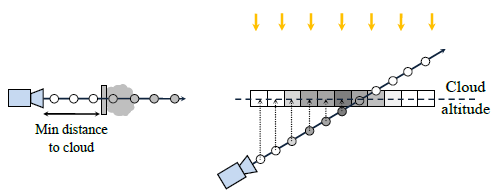
\includegraphics[scale=0.8]{images/integration.png}
\caption{Integration of clouds with the atmospheric light
scattering: attenuation along the view ray (left) and sun light
attenuation (right)}
\label{f17}
\end{center}
\end{figure}

At each ray marching step, we check if a point is above or under the cloud. If the point is under the cloud, the cloud density texture is sampled to get the occlusion by the cloud. Meanwhile, the transparency and distance to clouds in screen space are used to attenuate scattering along the view rays. There is one thing to be aware, in this step, the author made an assumption that the altitude the the cloud is fixed.

\section{Estimating Occlusion}
We already have the scattering data, by this point, the cloud is still semi-transparent no matter how thick it is. 
\subsection{The Design}
The occlusion describes the attenuation by other particles as the light travels to the current particle. Thus, computing the light occlusion is necessary.

\subsection{The Implementation}
\begin{figure}[htp]
\begin{center}
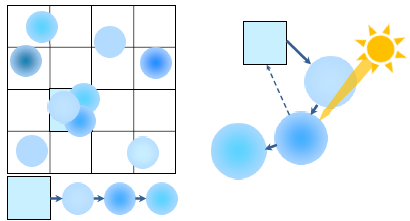
\includegraphics[scale=0.7]{images/occlusion.png}
\caption{Light-space tile grid (left) and computing light occlusion
by traversing the tile’s list (right)}
\label{f14}
\end{center}
\end{figure}

The occlusion is estimated in the following 3 steps:
\begin{enumerate}
\item Perform light-space tiling and construct lists of particles
covering each tile. In this step, one tile is actually one pixel, and each particle is assigned to one tile. A buffer of the screen size is used to store the index of the first particle in the list and another buffer is used to store the lists elements. As discussed in the first section of this chapter, it is important to preserve the original particle order for blending purpose. Hence, the Pixel Shader Ordering is used.
\item Traverse the particle lists from the previous step to estimate the occlusion. This step is carried out by the compute shader. Since each particle is assigned to one tile, the shader traverse through the list of the tile and calculate the opcity of particles on the light path. As the particles are in back-to-front order, the traversing loop for the compute shader can be terminated immediately when the current particle is reached. Or the programmer can set a threshold for the total transparency. The threshold makes sure that the cloud will never be totally semi-transparent at some certain transparency level. And it is encouraged to set a threshold for faster performance.
\item Smooth the occlusion and simulates the diffusion for the whole cloud. A compute shader is responsible for processing each valid particle and performing low-pass filtering of the light occlusion. The author also mentioned that using particle density as weights is a good way to avoid incorrect smoothing.
\end{enumerate}


\section{Generating Real-time Shading Model}
In this section, the author proposed with an approximated solution to Equation 2.9: $L(C, \vec{v}) = L_{In}(C, \vec{v}) + e^{-\tau(P_0, P_1)} \cdot L_B$ using the results from the previous two steps, which are the \textbf{optical depth} $\overline{T}$, the \textbf{single scattering} $\overline{L}_{in}^{(1)}$ and the multiple scattering $\overline{L}_{in}^{(M)}$.

To generate a shading model, the first step is getting the optical depth $\overline{\tau}$ for the given ray from $\overline{T}$:
\begin{equation}
\overline{\tau} = \overline{T}(\varphi_S, \theta_S, \varphi_v, \theta_v).
\end{equation}

\subsection{The Design}
The lighting model has three components: single scattering, multiple scattering and ambient. 

\begin{enumerate}
\item The author assumed that the single scattering $\overline{l}^{(1)}$ in the light model is equal to single scattering in the homogeneous sphere:
\begin{equation}
\overline{l}^{(1)} = P(\theta) \cdot \overline{L}^{(1)}(\theta_S, \phi_v, \theta_v, \overline{\rho} \cdot \overline{\tau}),
\end{equation}
where $\overline{\rho}$ is the density scale of each particle and $P(\theta)$ is this the phase function discussed in Chapter 2.

\item However, the multiple scattering only depends on the total density scale of the whole particle, the individual optical depth and phase function do not have any impact. Hence, the multiple scattering can be evaluated using the equation below:
\begin{equation}
\overline{l}^{(M)} = \overline{L}^{(M)}(\theta_S, \phi_v, \theta_v, \overline{\rho})
\end{equation}

\item The ambient light $\overline{l}^{A}$ is used to make the creases of the cloud slightly brighter than the edges influenced by the distance to the first cloud. And this distance is stored in the 4D look-up table $\overline{T}$. It is used at run time for the ambient light intensity of the sky.
\end{enumerate}
 
\subsection{The Implementation}
\begin{lstlisting}
void GetSunLightExtinctionAndSkyLight(in float3 f3PosWS,
                                      out float3 f3Extinction,
                                      out float3 f3AmbientSkyLight,
                                      Texture2D<float2> tex2DOccludedNetDensityToAtmTop,
                                      Texture2D<float3> tex2DAmbientSkylight )
{
    float3 f3EarthCentre = float3(0, -g_MediaParams.fEarthRadius, 0);
    float3 f3DirFromEarthCentre = f3PosWS - f3EarthCentre;
    float fDistToCentre = length(f3DirFromEarthCentre);
    f3DirFromEarthCentre /= fDistToCentre;
    float fHeightAboveSurface = fDistToCentre - g_MediaParams.fEarthRadius;
    float fCosZenithAngle = dot(f3DirFromEarthCentre, g_LightAttribs.f4DirOnLight.xyz);

    float fRelativeHeightAboveSurface = fHeightAboveSurface / g_MediaParams.fAtmTopHeight;
    float2 f2ParticleDensityToAtmTop = g_tex2DOccludedNetDensityToAtmTop.SampleLevel(samLinearClamp, float2(fRelativeHeightAboveSurface, fCosZenithAngle*0.5+0.5), 0).xy;
    
    float3 f3RlghOpticalDepth = g_MediaParams.f4RayleighExtinctionCoeff.rgb * f2ParticleDensityToAtmTop.x;
    float3 f3MieOpticalDepth  = g_MediaParams.f4MieExtinctionCoeff.rgb      * f2ParticleDensityToAtmTop.y;
        
    // And total extinction for the current integration point:
    f3Extinction = exp( -(f3RlghOpticalDepth + f3MieOpticalDepth) );
    
    f3AmbientSkyLight = tex2DAmbientSkylight.SampleLevel(samLinearClamp, float2(fCosZenithAngle*0.5+0.5, 0.5), 0);
}
\end{lstlisting}
This function \textbf{GetSunLightExtinctionAndSkyLight} basically calculate the ambient sky light \textbf{f3AmbientSkyLight} from the look-up table $\overline{T}$. As we can see, we get the earth center position \textbf{f3EarthCentre} first, and use it to calculate the distance between the earth center to the particle \textbf{fDistToCentre}. Then, the altitude of the particle \textbf{fHeightAboveSurface} and the cos value of the zenith angle \textbf{fCosZenithAngle} are evaluated. After this, we retrieve the optical depth from the pre-computed 4D look-up tale. Finally, we calculate the ambient sky light using the data from above and sample it with a 2D texture describing the general ambient pattern.

\section{Volume-Aware Blending}
The author proposed with a new blending method because the traditional alpha blending is not able to describe the intersection of particle volumes.
\subsection{The Design}
The figure below shows a typical intersection scenario of two particles. The particles have non alpha-premultiplied colors $C_0, C_1$ and densities $\rho_0, \rho_1$.

\begin{figure}[htp]
\begin{center}
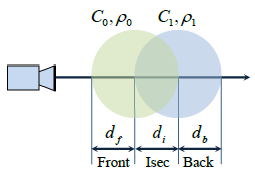
\includegraphics[scale=1.0]{images/intersection.png}
\caption{Intersection of two volumetric particles}
\label{f15}
\end{center}
\end{figure}

The author derived the transparency and color for the 3 parts:
\begin{enumerate}
\item Front:
\begin{eqnarray}
T_f &=& e^{-\rho_0 \cdot d_f \cdot \beta}\\
C_f &=& C_0 \cdot (1-T_f)
\end{eqnarray}

\item Back:
\begin{eqnarray}
T_b &=& e^{-\rho_0 \cdot d_b \cdot \beta}\\
C_b &=& C_0 \cdot (1-T_b)
\end{eqnarray}

\item Intersection:
\begin{eqnarray}
T_i &=& e^{-(\rho_0+\rho_1) \cdot d_i \cdot \beta}\\
C_i &=& \frac{C_0\rho_0 + C_1\rho_1}{\rho_0+\rho_1} \cdot (1-T_i)
\end{eqnarray}
\end{enumerate}

Hence, the final transparency and alpha-premultiplied color are:
\begin{eqnarray}
T &=& T_f\cdot T_i\cdot T_b\\
C &=& C_f + T_f \cdot Ci + T_f \cdot T_i \cdot C_b
\end{eqnarray}

\subsection{The Implementation}
The author mentioned that current graphics hardware has no programmable blending unit. Thus, he used an extension from Intel called \textbf{Pixel Shader Ordering} to solve the above equation, which is able to read and write to arbitrary memory location. The author used two buffers to do the implementation, and they are UAV buffer and back buffer.

\begin{figure}[htp]
\begin{center}
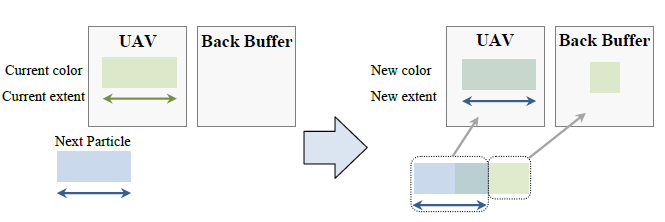
\includegraphics[scale=0.8]{images/uvabuffer.png}
\caption{Updating UAV and back buffer during the
volume-aware blending}
\label{f16}
\end{center}
\end{figure}

The implementation details can be narrowed down into 3 steps:
\begin{enumerate}
\item Enable Pixel Shader Ordering.
\item Store the current particle's color, density and min/max extent into the UAV buffer.
\item Check each new particle against the currently one in the UAV buffer. If the new particle is in front of the current particle, the current is blended into the back buffer and replaced with the new one. If the new particle overlaps with the current particle, they are blended and stored into the back buffer.
\end{enumerate}

\section{Conclusion and Review}
This chapter describes the essential algorithms and implementations of the proposed method from the paper. We looked into how the particles are generated, how the 4D look-up tables are computed, how the optical depth and scattering are computed and stored, how the occlusion is estimated, how the real-time shading model is generated, and finally, how the volume-aware blending is approached.

The architecture of this method is absolutely designed after carefully consideration. Overall it's efficient and able to output a realistic result of simulating the cumulus clouds. After reading the article for several times and inspecting the source, I have some suggestions to improve the method.

\begin{enumerate}
\item The author used 4 angles to describe a ray when computing the optical depth and scattering. This approach is straight forward, but not so efficient. Consider this, using one quaternion to describe the start point of the ray, and another quaternion to describe the ray direction. And by interpolating these two quaternions, we can describe each possible ray in the sphere with some certain sampling level.

\item When computing the scattering, the author assumed that the light source is always a directional light, which in the common case is the sun. So when doing the integration of the final light through the cloud, the distance from the particle to the light source is not considered to be changing. And this is not true. Here is a typical scenario, an aircraft flies above the cloud in the night, and the only light source will be the point lights from the pilot lamps of the aircraft. So in my opinion, the author should extend the light source in order to adapt the clouds into different situations.

\item When generating particles, performing volume-aware blending and any operations to the particles, they have to be sorted. Sorting millions of particle costs a heavy load of calculations. In my opinion, when generating the particles, make sure they are not intersected with each other will be another cheap solution. Although we could the lose the feature of volume-aware blending, but the outputting the result will be more fast, and it can be applied into real time games or simulators.

\item  When computing optical depth and scattering, we noticed that there are lots of duplicated operations of decomposing the projection plane and the 4D look-up table to calculate the ray. If we design a specific data structure for the information of a ray, the redundancy problem can be solved.

\item When integrating with the atmospheric scattering, the author assumed that the clouds will always have constant altitude, which is not always true. Actually, a clouds has its own physical attributes, e.g. the saturation of water drops will affect the density of the cloud, and further more, it affects the altitude of the cloud. If we want to the clouds behave differently in various weather conditions, changing the altitude when integrating with atmospheric scattering has to be considered and implemented.

\item The camera is always outside the clouds, which means the user is not able to interact with the clouds. We noticed that, in the pre-computing steps, the light inside the clouds is not stored in the 4D look-up table. I suppose that is due to the consideration of the limitation of memory space.
\end{enumerate}
